\documentclass[border=10pt]{standalone}
\usepackage[svgnames]{xcolor}
\usepackage{amsmath}
\usepackage{pgfplots}
\pgfplotsset{compat=newest}
\usepackage[sfdefault]{FiraSans}
\usepackage{FiraMono}
\renewcommand*\familydefault{\sfdefault}
\begin{document}
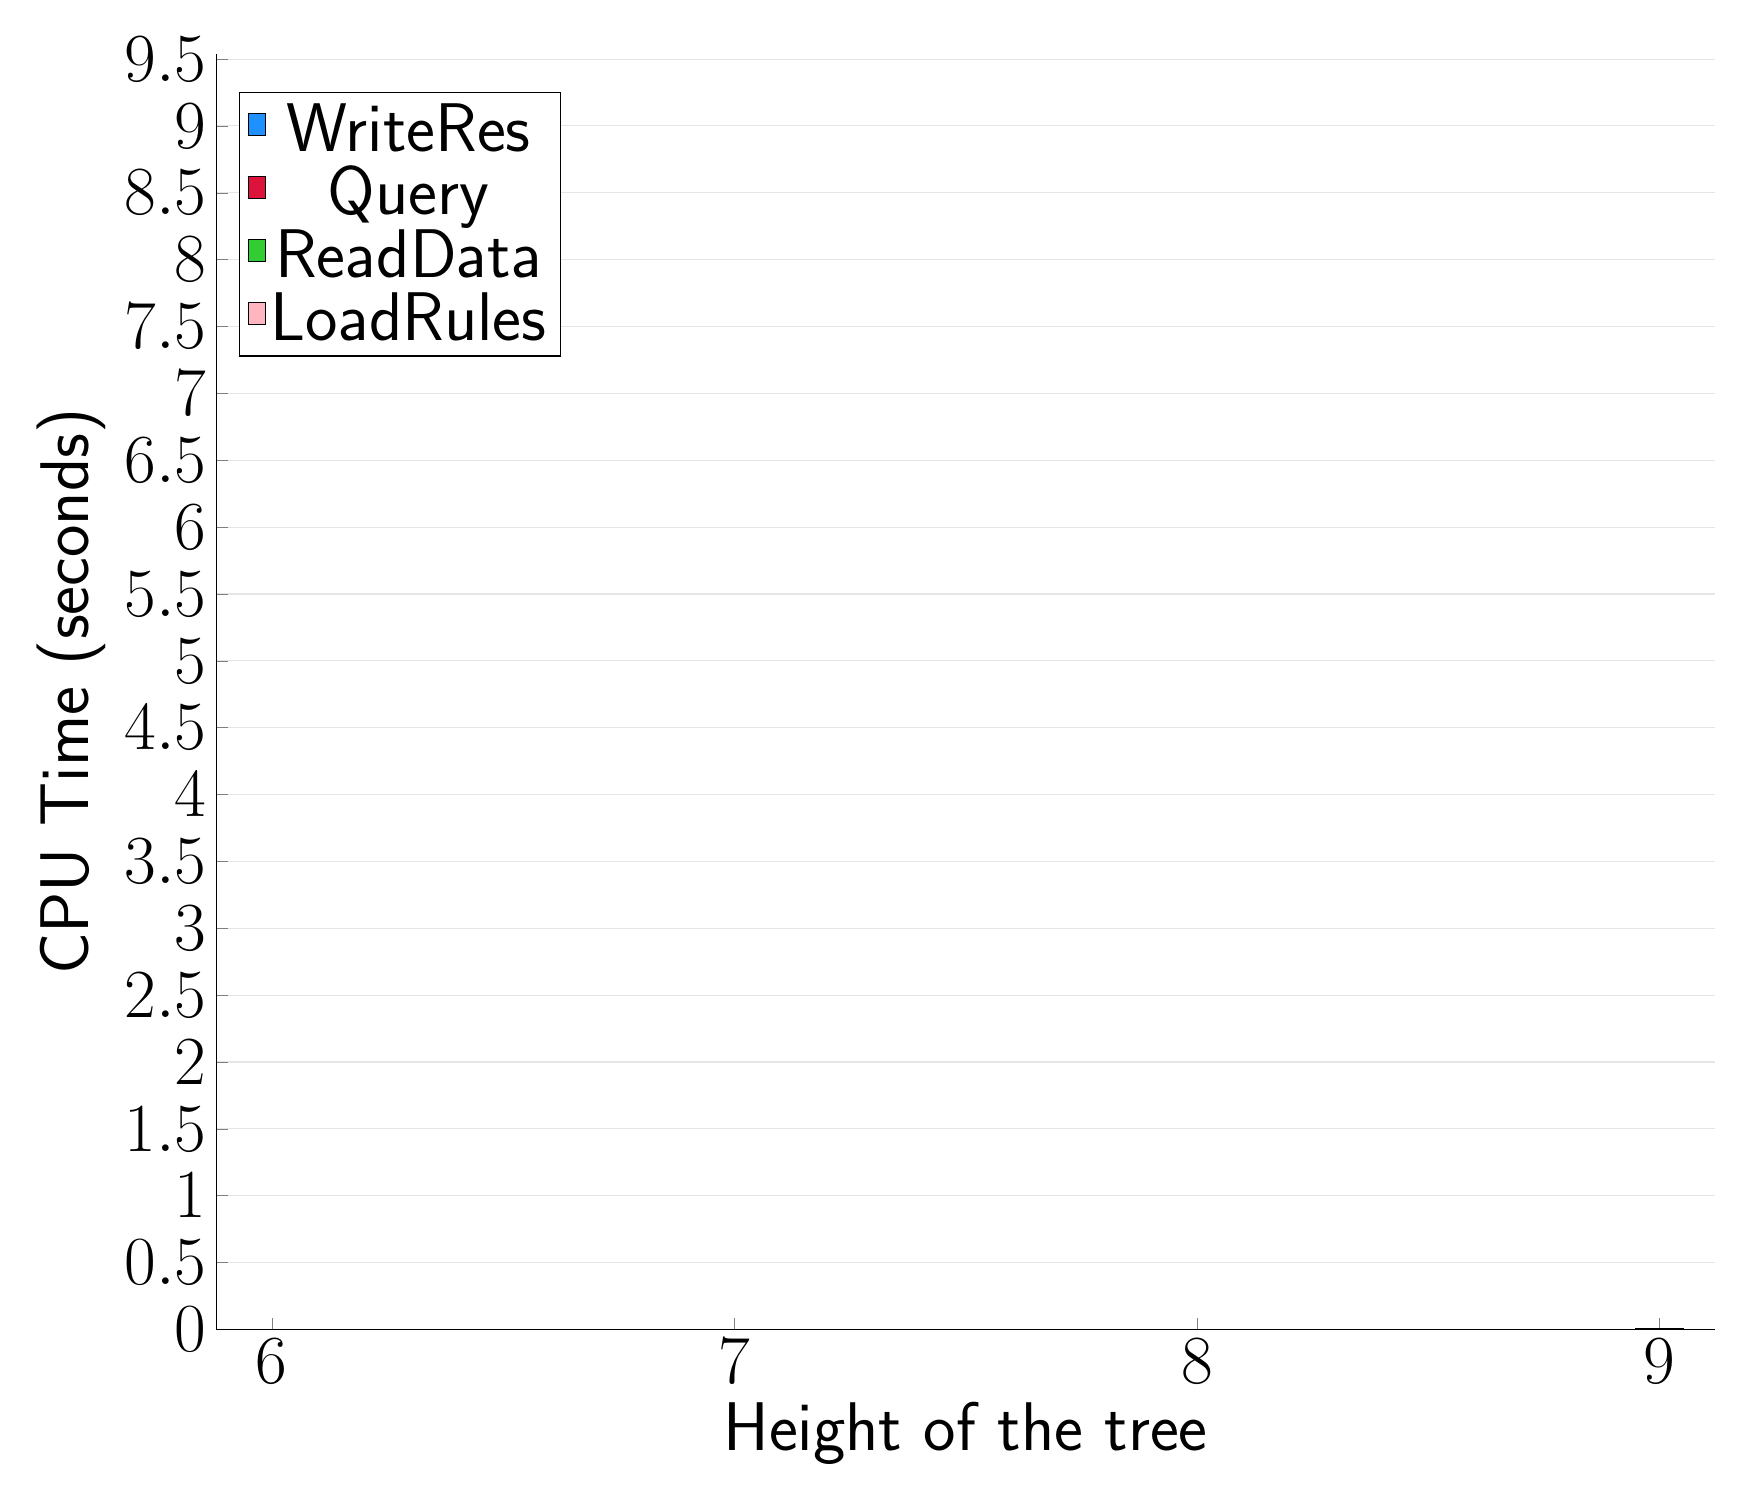
\begin{tikzpicture}
\begin{axis}[
   ybar stacked,
   width=1.7\textwidth,
   bar width=0.6cm,
   ymajorgrids, tick align=inside,
   major grid style={draw=gray!20},
   xtick=data,
   ymin=0, ymax=9.538,
   axis x line*=bottom,
   axis y line*=left,
   enlarge x limits=0.04,
   legend style={
       at={(0.23, 0.97)},
       anchor=north east,
       legend columns=1,
       font=\Huge,
   },
   ylabel={CPU Time (seconds)},
   xlabel={Height of the tree},
   label style={font=\Huge},
   tick label style={font=\Huge},
]
\addlegendimage{fill=DodgerBlue, draw=black, line width=0.2pt}
\addlegendentry{WriteRes}
\addlegendimage{fill=Crimson, draw=black, line width=0.2pt}
\addlegendentry{Query}
\addlegendimage{fill=LimeGreen, draw=black, line width=0.2pt}
\addlegendentry{ReadData}
\addlegendimage{fill=LightPink, draw=black, line width=0.2pt}
\addlegendentry{LoadRules}
\addplot +[fill=LightPink, draw=black, line width=0.55pt] coordinates {
(6, 0.0005516)
(7, 0.0005606)
(8, 0.0005587999999999999)
(8, 0.0005538000000000002)
(8, 0.0005529999999999996)
(9, 0.0005533999999999998)
(9, 0.0005599999999999998)
(9, 0.0005518000000000001)
(9, 0.0005519999999999996)
(9, 0.0005543999999999998)
};
\addplot +[fill=LimeGreen, draw=black, line width=0.55pt] coordinates {
(6, 0.0001772000000000004)
(7, 0.00022539999999999981)
(8, 0.0003226000000000004)
(8, 0.0003288)
(8, 0.00032180000000000045)
(9, 0.0005254000000000003)
(9, 0.0005268)
(9, 0.0005337999999999997)
(9, 0.0005278000000000001)
(9, 0.000526)
};
\addplot +[fill=Crimson, draw=black, line width=0.55pt] coordinates {
(6, 3.2000000000000778e-06)
(7, 3.0000000000005744e-06)
(8, 2.7999999999996784e-06)
(8, 3.2000000000000778e-06)
(8, 2.800000000000374e-06)
(9, 3.200000000000426e-06)
(9, 3.0000000000002262e-06)
(9, 3.0000000000002262e-06)
(9, 3.19999999999973e-06)
(9, 3.2000000000000778e-06)
};
\addplot +[fill=DodgerBlue, draw=black, line width=0.55pt] coordinates {
(6, 6.140000000000035e-05)
(7, 6.039999999999934e-05)
(8, 5.94000000000001e-05)
(8, 5.939999999999974e-05)
(8, 6.079999999999906e-05)
(9, 5.9599999999999246e-05)
(9, 6.099999999999998e-05)
(9, 6.0999999999999247e-05)
(9, 5.960000000000031e-05)
(9, 6.05999999999999e-05)
};
\end{axis}
\end{tikzpicture}

\end{document}
